\documentclass[11pt]{article}
\usepackage{rotating}
\usepackage{geometry}

\makeatletter

    \def\ps@titlestyle{
        \let\@oddhead{(0pt,0pt){}{}{}(\textwidth,1pt)}
        \let\@evenhead{(0pt,0pt){}{}{}(\textwidth,1pt)}
        \def\@oddfoot{(\textwidth,1pt){}{}{\coursecode\hfill\pagemark}(0pt,0pt)}
        \def\@evenfoot{(\textwidth,1pt){}{}{\coursecode\hfill\pagemark}(0pt,0pt)}
    }

    \renewcommand\maketitle{
        \clearpage
        \newgeometry{left=2.5cm,right=2.5cm,top=7cm,bottom=3cm}
        \begin{center}
            \vspace*{\baselineskip}
            \huge{\textbf{\@title}} \\ [2ex]
            \Large{\@author \space (\@registration)} \\
            \Large{\@coursecode} \\
            \vspace*{\fill}
        \end{center}
        \restoregeometry
        \clearpage
    }

    \newcommand*{\coursecode}[1]{\renewcommand*{\@coursecode}{#1}}
    \newcommand*{\@coursecode}{\ClassError{error}{No \string\coursecode\space given}{}}

    \newcommand*{\registration}[1]{\renewcommand*{\@registration}{#1}}
    \newcommand*{\@registration}{\ClassError{error}{No \strin\gregistration\space given}{}}

    \newgeometry{left=2.5cm,right=2.5cm,top=3cm,bottom=3cm}

\makeatother


\title{Unity Games Development: Design and Plan}
\author{Zack Langley}
\coursecode{CMP-6056B}
\registration{100394283}


\begin{document}

\thispagestyle{empty}
\maketitle

\thispagestyle{empty}
\tableofcontents

\graphicspath{ {./images/} }

\clearpage

\setcounter{page}{1}

\section{Introduction}
With several development sprints having been completed for the game so far, progress in various 
areas has been achieved to a level sufficient enough for this document to outline the implemented 
systems and discuss their purpose and relevancy within the entire project. Clear justification and
honest evaluation for the current systems within the game will improve the organization of future 
development and allow for a more straightforward implementation of any remaining systems. 
Furthermore, the highlighting of currently implemented features will provide a great visualisation 
and outline for what is to be expected of the game in its final state. \\

\section{Overview}
The game is a first-person wave shooter with a built-in economy system, multiple different maps and
a variation of in-game objectives, providing diverse and unique gameplay experiences with every 
attempt. The game takes many elements from action and shooter games in order to situate itself 
properly within those genres, while also employing minor elements from games within the horror 
genre as a way to bring together overarching thematic choices by providing them with an adequate
degree of context. While still important, the aforementioned horror elements will be minimal as to
not detract from the genres at the forefront of this game. Nonetheless, the balance of these 
genres is largely appropriate for the entire game at hand. \\

\subsection{Core Concepts}
The ability for the core game to be replayed many times to a maintained, enjoyable standard is
imperative to its success. Massive effort and thought were placed into constructing the outline for
the games core gameplay loop that would be at the root of all the experiences each player will have
with this game. Progress within the game revolves around earning currency and using it to better
the player so that they may then survive for longer, either through player upgrades of some kind or
through expansion of the area available to the player. This cycle will then repeat, with enemies
growing in difficulty as the waves progress in order to incentivise the player to make the
necessary improvements. In order to implement this loop effectively, the player must start within a
confined area of the map and should only be granted a basic arsenal that is sufficient enough to
earn currency. This loop will remain consistent, even when other aspects of each replay are
altered, such as what map is being played or what final objective the player is working towards.

The most apparent objective to the player will be to simply progress through the waves in an
attempt to obtain the highest possible wave that they can. This will ultimately be a test of
endurance for the players that will promote close investigation into many areas of the game in
order to locate new optimisations and strategies in order to make the process of obtaining higher
waves more efficient. Although out of scope for the project, a great way to accentuate this system
would be to include a variation of a leaderboard system that would allow players to share their
highest achieved waves with everyone.

Another objective that will be provided to the player will be the unique questlines implanted into
the individual maps within the game. Featuring multiple smaller steps, the questline will offer a
separate challenge that will take place across the entire map and will attempt to thoroughly test
the players ability to solve puzzles and find the next possible steps. This will offer a more
linear experience for the players that find that to be more preferable than the more arcade-like
playstyle offered by the standard wave system, which will not be forgotten even if the player is
focused on the questline. It will be required of the players to balance both as a test of their
abilities and to not alter the game too much in an attempt to maintain its core identity.
Nonetheless, the questlines available will be completely optional in an attempt to not detriment
the experience for all players.

Smaller objectives, similar in nature but entirely unrelated to the questline, will also be present
in the games maps for the player to find and complete. These will be intended to only provide the
player with small benefits within that replay, having little impact outside of that or on the game
as a whole. While rather inconsequential, this does add to overall level of content available to
player during any replay.

Ample levels of side content can provide fresh and new experiences for players for a large amount
of time, making the game much more worthwhile for them to dedicate their time to for any quantity
of time. The combination of all progression methods should be able to achieve the desired result of
providing players with varied experiences for a long period of time. Even when all has been
discovered by the player, the core systems of the game have been constructed in a manner that
encourages the player to replay and continue to enjoy the game, free of tedium and boredom for any
of the many different types of players that may gravitate to the game. \\

\subsection{Inspiration}
The game takes inspiration from many others within the genres it has placed itself within. As such,
heavy attention was given to other first-person shooter titles, especially those that overlap with
the horror genre in the same manner this game does. Three games are notable in providing heavy
inspiration to this game, with those being Left 4 Dead, Sker Ritual and Call of Duty. The most
influential of these is Call of Duty, however specifically the titles within the franchise that
contain some variation of their Call of Duty: Zombies alternative game mode. While not a standalone
game, the game mode has become very popular and is very similar to the proposed outline for this
game. Figure \ref{fig:inspo} is an image taken from within one of the games in this franchise and
will serve as a point of reference when constructing select systems for this game. \\

\subsection{Unique Features}
In order for this game to successfully come together it must be unique and not just a copy of one
of the games that it is inspired be. For this to be achieved, development of the game will take
more care to improve the versatility of the game, making it more accessible and appealing to a
wider audience. Furthermore, the systems inspired by other games will be altered enough to provide
a definitively unique experience that would not be achieved by playing any of those games. \\

\subsection{Target Audience}
Another aspect of the games that inspired this one that can be translated over is their target
audience. Being situated within the same genres, the predominant target audiences will be fairly
similar to one another. The target audience for a first-person shooter game is young men aged
between 15 and 35. The people that are most likely to be interest in this game will likely fit
into this demographic, however there is hope that the scope of the target audience will be further
expanded due to the diverse gameplay attempting to be constructed by this game. \\


\section{Design}
The game will utilise an increasing popular visual style in the modern game development landscape,
in which low poly models are used in conjunction with impressive lighting and digital effects. 

The use of low poly 3D assets provides many benefits to development. As they are becoming
increasingly popular, they are easy to locate and acquire from online marketplaces. If something is
not found on an online marketplace, it could potentially instead be constructed from scratch.
Furthermore, low poly assets grant better performance to the game and reduce the final file size.
The lighting and effects previously mentioned will be used to highlight and accentuate the models
and the constructed environments. When they are all combined together well, they create something
very visually appealing. \\

\subsection{Engine}
Unity was the engine chosen to develop this game, with the choice being made very early on. The
biggest reason for using Unity over any of the other options was ultimately the foundation of
support that it had and the accessibility of that support. Within lecture and lab content, there is
a greater level of knowledge and support for Unity development. Furthermore, there is a surplus of
tutorials, documents and other resources that can be found very quickly online. These reasons made
Unity appear to be the sensible and secure option for the development of this game. Beyond this,
the scale of the game aligned closely with the scale of other popular games also developed in
Unity. It appeared to be the best option for the balance of scale and performance. 

Unreal Engine was also a contender for the game engine to be used. Unreal contains many of the same
feature, accessories and systems that are found within Unity. Furthermore, Unreal has shown to be
very impressive in creating large scale, AAA \footnote{AAA or Triple-A refers to games made with a
high budget and using a large development team.} games. On the other hand, personal usage and
experience with the new version of Unreal Engine have allowed me to conclude that it would not be
the most suitable option for the game. Unreal Engine 5 is a much larger engine than any of the
others considered for this game. It is known to create final products with a much larger file size,
something that was substantially different from the direction this game needed to be taken in.
Lastly, support for Unreal is still plentiful, however the support within the in-person sessions
would be less than that of Unity. It is because of these factors that Unreal Engine was not
considered further as a potential candidate for this game’s engine.

The last potential option considered for the game was the Godot Engine. Godot is a free and
open-source game engine, making it very appealing for many – especially those developing
independently. Furthermore, it is incredibly lightweight while still containing an impressive set
of features for development. Although there are a large number of positives, Godot support in
person was going to be non-existent and as such, development using it could potentially become
very difficult with no support to help realign the project. 

Upon review of all the possible engines and weighing their positives and negatives, Unity was the
engine that best aligned with the game as a whole. It will be able to continue to support the
expansion of the game through development and can do so effectively and efficiently. The large
collection of support for Unity means that development will be able to effectively move past any
issues and continue with minimal overall disruption. \\

\subsection{Story}
As it currently stands, the story and background of the game has not yet been fully developed as it
is less important that the implementation of the many foundational systems. Nonetheless, it has
been given some degree of thought. 

Environmental storytelling is an impressive way to provide essential story information to the
player and improve the maps within the games, making them feel more relevant and tied together.
This would be the ideal method of imparting story information onto the player. 

Using other methods, such as pages of text for the player to read, detract from the gameplay and
take the player out of their immersive state. While sometimes necessary to give information in a
similar manner, it will be minimised in this game and will be done in the best possible way in
order to not detract from the gameplay or potentially confuse the player. \\

\subsection{Controls}
In the modern gaming landscape, there are an abundance of well-designed first-person shooter
games. This has resulted in a great standard being found for the control schemes used within
these games, which can then be taken and implemented into this game. The benefit of this is that
players will be able to quickly pick up the control scheme and play confidently, as they would in
many other first-person shooter games. 

Currently in development, this control scheme is the extent of what has been implemented, however
further plans are in place to expand on the control system. Support for controllers is very
important, as it is common for a players preferred way to play a first-person shooter to be with a
controller. Furthermore, allowing for controller support will hopefully allow for a greater degree
of accessibility within the game, as controllers are sometimes not just a preference but instead a
necessity in order for some players to experience the game to any degree. 

The final planned aspect relating to the control system is a fully customisable set of controls
that would allow the player to remap their actions to whatever buttons they desire. This will
provide the player with an even greater level of accessibility support and should allow for anyone
to play the game in the way they prefer or require. \\

\subsection{Levels}
To provide the player with a greater level of opportunities when playing the game, there will be
multiple maps available to play. All will be thematically different and mostly disconnected to one
another in order to provide unique experiences within each. Nonetheless, they will all serve the
same general purpose and feature the same core gameplay loops. Furthermore, the inclusion of
thematically distinct maps will help to widen the scope of people that may be interested in the
game. In order to achieve the goal of having many maps within the game, they will be of slightly
smaller scale. This will be done to a level that is not a detriment to the overall experience of
the map itself or the game as a whole but that will also allow for a more streamlined development
experience of the maps. \\

\subsection{User Interface}
The design of any menu or UI element within the game will follow a set design pattern,
being modern, angular and flat. This is not only to be clear and straightforward but to also be
thematically consistent with the other graphical elements of the game.

The menus within the game will be constructed to be clear and effective. Relevant information and
sub-menus will be grouped together correctly and not unnecessarily, in order to prevent there being
difficulties locating certain areas. Menu control systems will be inspired by other modern games,
allowing for appropriate and fluid movement between menu locations. 

UI that appears during gameplay will also need to be clear and concise in order to not detract from
the rest of the game. This will entail a well-designed and minimalistic HUD for the player and not
much else. The HUD will provide the player with the essential gameplay information that would be
impractical to show anywhere else. \\

\section{Implementation}
As it currently stands, only a select number of fundamental systems have been implemented into the
game. These have so far established the game correctly as a first-person shooter, with other
aspects yet to be implemented to full encompass the entire foundation of the game. \\

\subsection{Player}
The first and arguably the most important feature to be implemented into the game was the player
themselves. This began with creating a rudimentary model and adding a camera that would allow the
player to view the preliminary testing level. Controls were then implemented to allow for movement
of the camera from mouse input. Further additions were added in order to make the camera behave
more like any other first-person camera would, such as clamping the angle the camera can move when
looking up and down. 

Once camera controls were implemented, player movement was next. A simple script was created that
allowed the player to move horizontally, taking advantage of the Unity input manager. Once this
felt complete, jumping and sprinting were added in order to expand the available movement options.
The implementation of jumping entailed adding a small collider to the base of the player model that
would check if the player was touching the floor, allowing them the opportunity to jump. Sprinting
detects if the left shift key is being held down and if so, provides a small movement speed
increase to the player. The values for all the individual movement components needed to be fine
tuned, however they are now in a good place and provide a well rounded and adequate first-person
character controller. 

The last major implementation relating solely to the player is the player UI. Rudimentary UI was
given to the player in order to gauge the effectiveness of their proposed design and highlight any
issues that there may be. Nonetheless, it assists in making the character feel much more like those
in other first-person shooter games. The design of the UI can be seen in figure
\ref{fig:ui-mockup}, with its current level of implementation being seen in figure
\ref{fig:weapon}. \\

\begin{figure}[htb] 
    \centering
    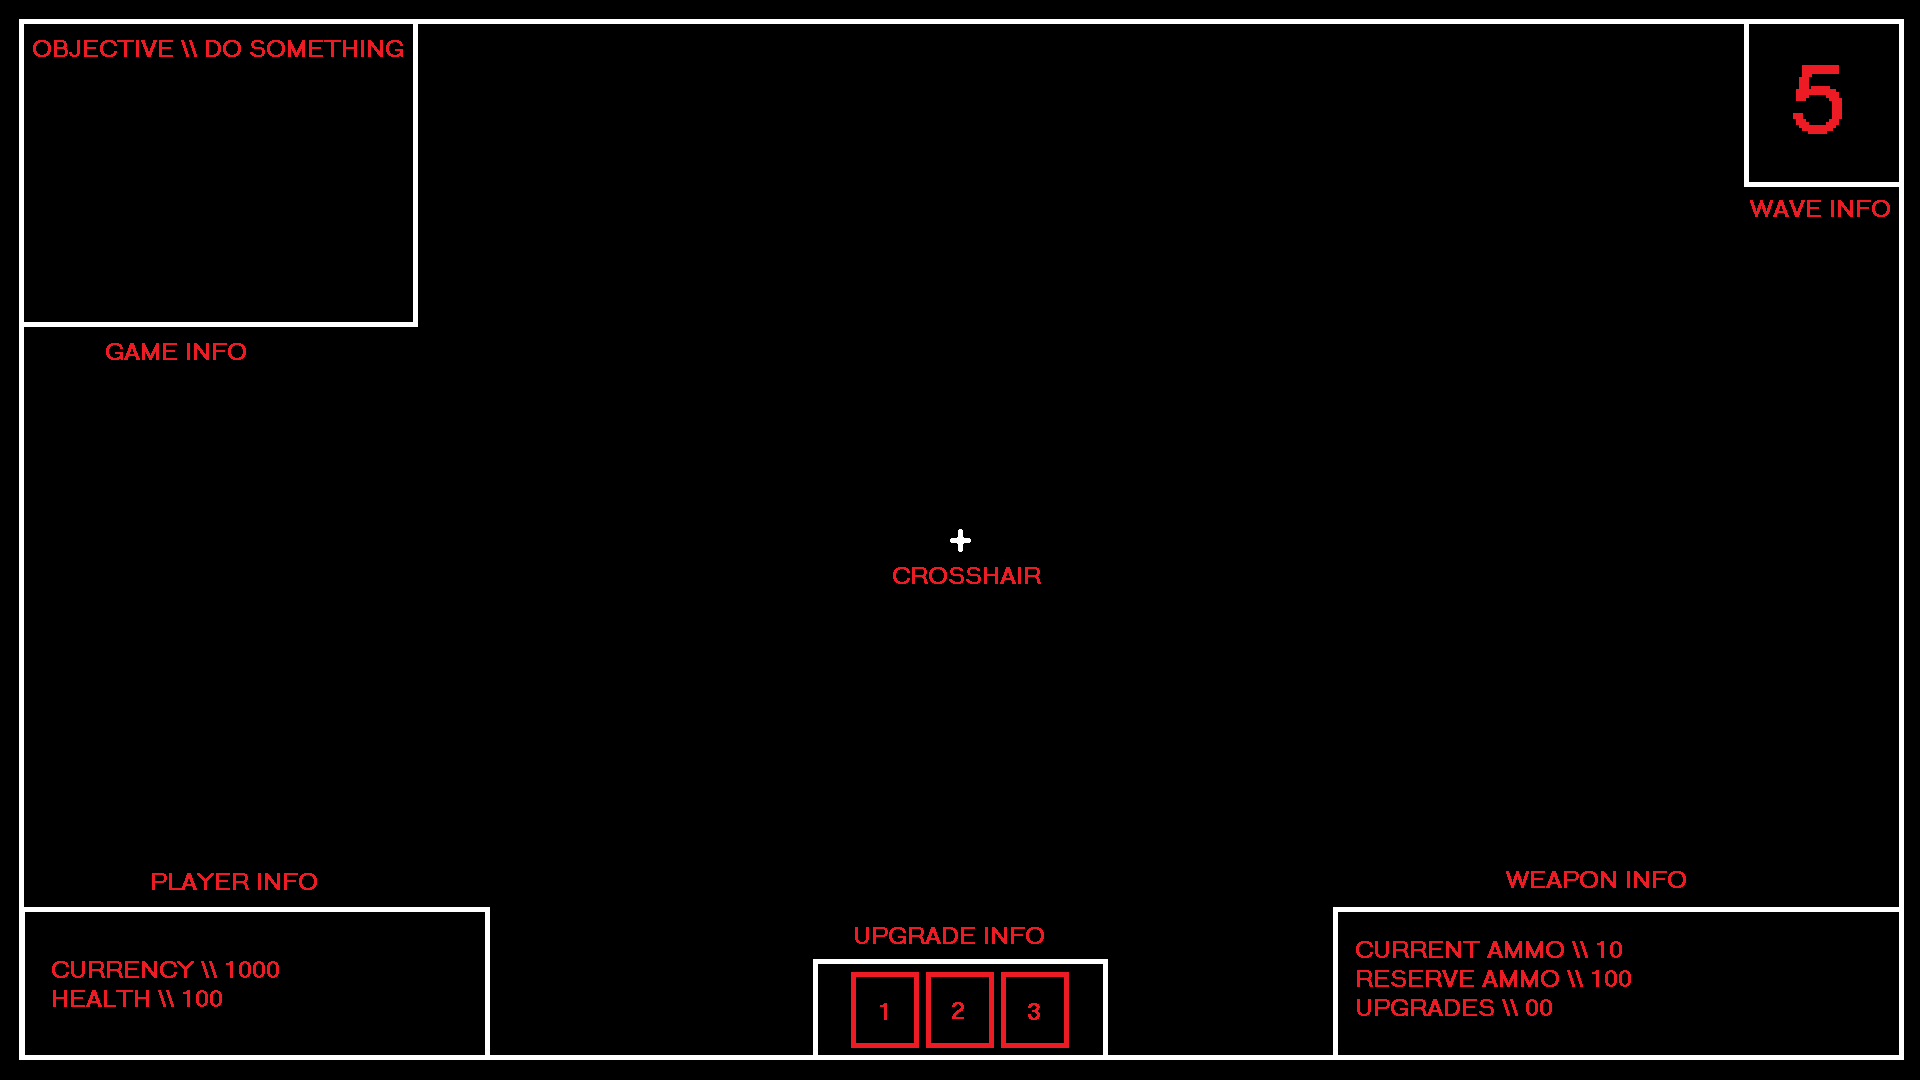
\includegraphics[width=\columnwidth]{ui-mockup}
    \caption{Mockup design of the player UI.}
    \label{fig:ui-mockup}
\end{figure}

\subsection{Enemy}
Enemy systems were implemented after the player had been completed. Similarly to the player,
rudimentary 3D models were constructed in order to serve as a representation of the enemy. This was
then followed by the functionality of the enemy, beginning with the UI that would be used to convey
essential information about the enemy to the player during gameplay. 

A health bar system was created in order to indicate to the player how much damage the enemy has so
far received. In order to maintain its effectiveness, it was ensured that the health bar would
always face the player head on in order to avoid the possibility of the information being
interpreted incorrectly due to distortions. Furthermore, the health bar only activates when there
is an update to the enemy’s health. This helps to minimise visual pollution at any given time,
reducing the information always being given to the player in an attempt to prevent them from being
overwhelmed.

\begin{figure}[htb] 
    \centering
    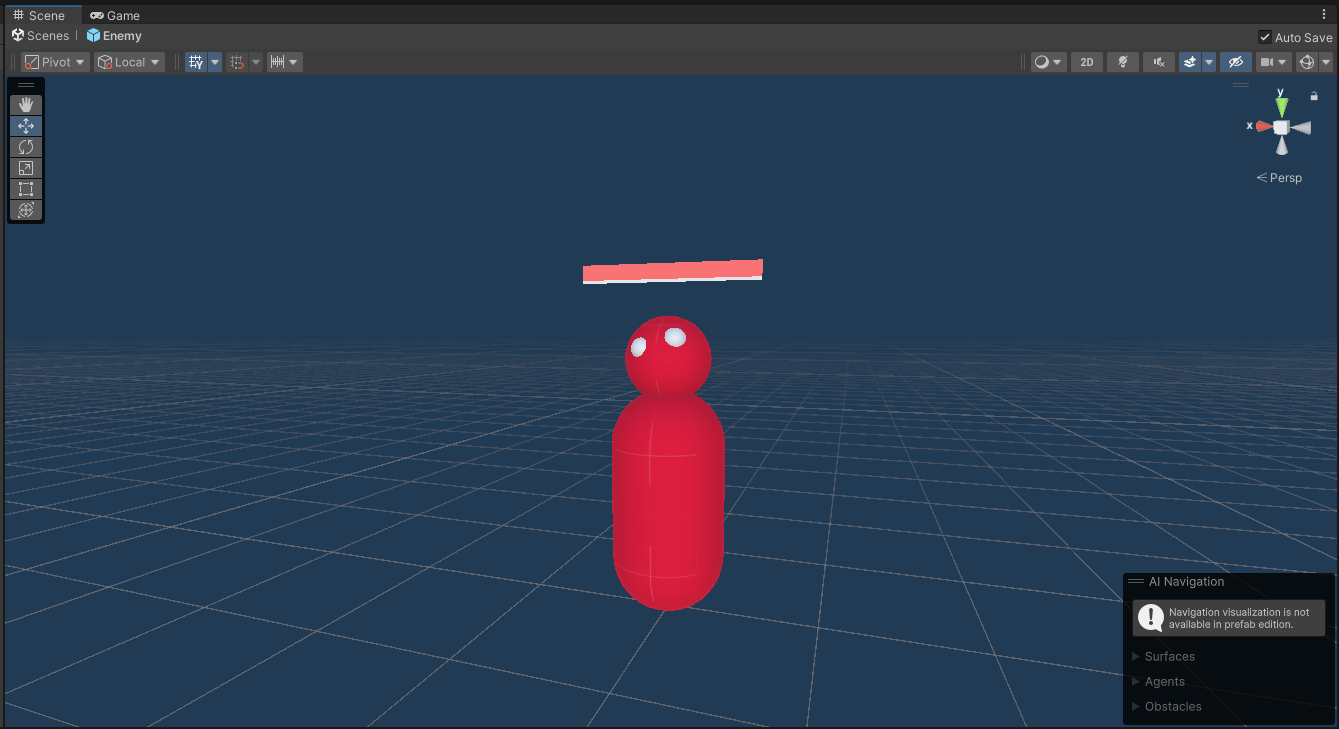
\includegraphics[width=\columnwidth]{enemy}
    \caption{Enemy model with healthbar system.}
    \label{fig:enemy}
\end{figure}

The other major system implemented for the enemy was its artificial intelligence, used
predominantly to locate and move to the position of the player. Utilising the navigation systems
available within Unity, the enemies were assigned the role of an agent with the player as their
target. A navigation mesh was then constructed using the current level geometry being used,
allowing for the enemy to traverse effectively. The efficiency of this system was also improved
through the utilisation of the A* algorithm in helping the enemy locate the player. \\

\subsection{Combat}
Combat systems could begin development after adequate player and enemy systems had been
implemented. Initially, this consisted of constructing a very basic representation of a weapon for
the player to hold which can be seen in figure \ref{fig:weapon}. After this, functionality could be
implemented. This consisted of a script that detects player button input, fires a ray cast and
detects what has been hit by it. This would allow for signals to be sent to the recipient so that
the event could be handled within the relevant script. 

The script makes use of a weapon class that was constructed. The weapon class was built from the
ground up to be easily adaptable and modular, as to make the addition of future weapons or the
modification of current ones easier. The class contains several modifiable fields for the weapons
attributes and statistics, such as the damage, the range, the rate of fire and if the weapon is
fully automatic or not. This is all taken into consideration by the combat script.

A comprehensive health system was then fully constructed and given to the player and enemies. This
health system is what handles the signals sent by the other facets of the combat system, correctly
applying information like the damage. Furthermore, the health system is able to make distinctions
between the area of the entity that has received damage. This allows it to calculate damage
modifiers if necessary, such as if an enemy has received damage to its critical location. As is
common for many other first-person shooter games, the critical location on enemies was chosen to be
their head. \\

\subsection{Levels}
An appropriate testing level was constructed in order to validate and confirm the functionality of
new systems. While not complex, it features large amounts of randomly places walls that were useful
in testing the effectiveness of the navigation of the enemy AI. It can be seen in figure \ref{fig:testing-map}.

\begin{figure}[htb] 
    \centering
    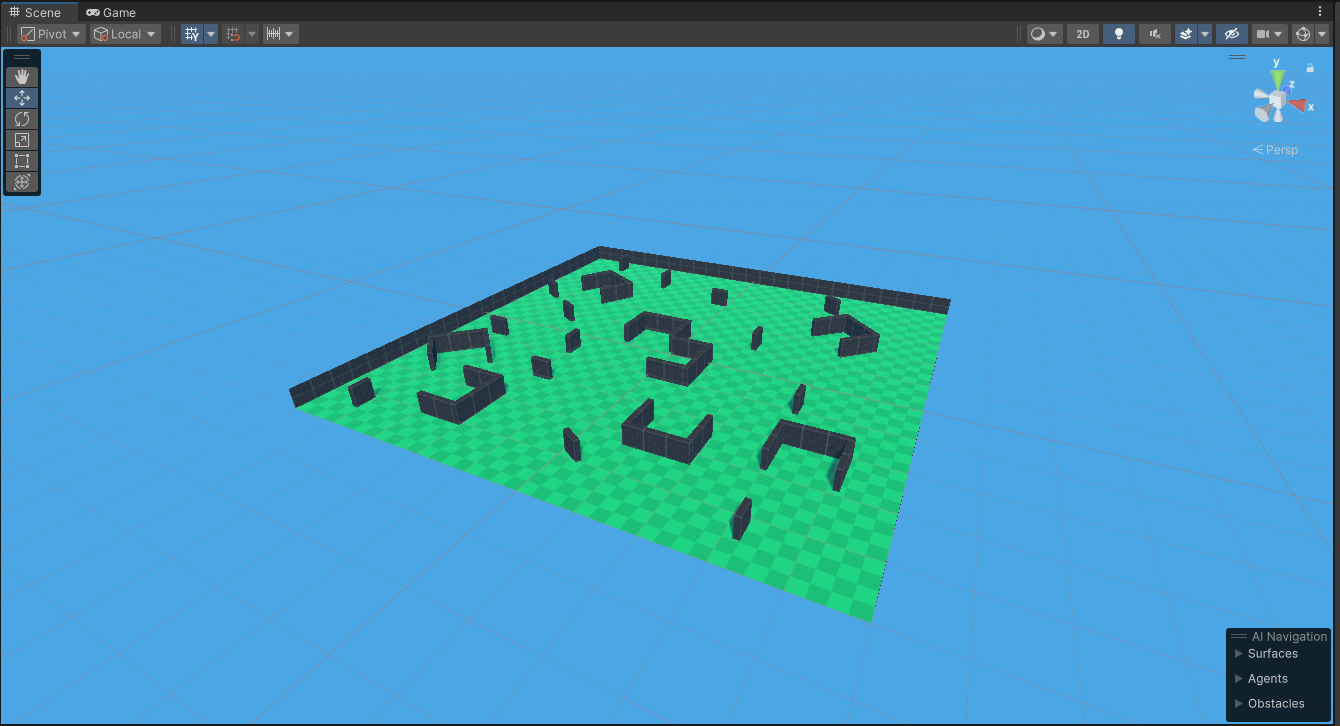
\includegraphics[width=\columnwidth]{testing-map}
    \caption{View of the testing map from above.}
    \label{fig:testing-map}
\end{figure}

A basic and grey-boxed \footnote{Grey-boxing is the process of building a prototype of the level
geometry to a playable version, usually constructed only with grey boxes.} version of the first
level ‘Farm’ has also been constructed, using a rudimentary blueprint made specifically for it that
can be seen in figure \ref{fig:farm-bp}. It can currently be played and is as effective as the
testing map, however is visually lacking compared to what the final version of the map is to be.
Nonetheless, it can be seen in figure \ref{fig:farm-map}. \\

\section{Conclusion}
The development of the game is in a very appropriate place for the time that has so far been spent.
With the correct pacing being continued from this point, all required features will be implemented
within reasonable time frames, allowing for additional time to be spent ensuring that all systems
are working together as intended and giving the final product other essential testing and
cleaning. \\

\clearpage


\appendix

\section{Image Gallery}
\begin{figure}[htb] 
    \centering
    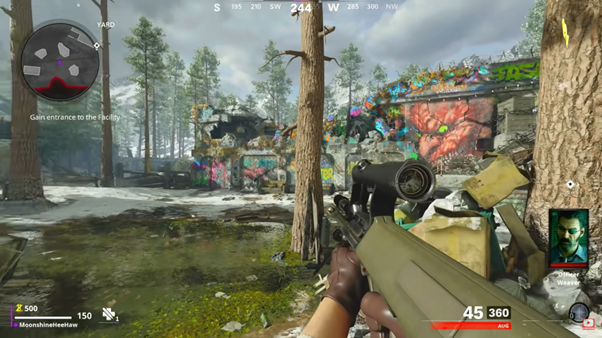
\includegraphics[width=\columnwidth]{inspo}
    \caption{A screen capture from \textit{Call of Duty: Black Ops Cold War}'s Zombies game mode.}
    \label{fig:inspo}
\end{figure}

\begin{figure}[htb] 
    \centering
    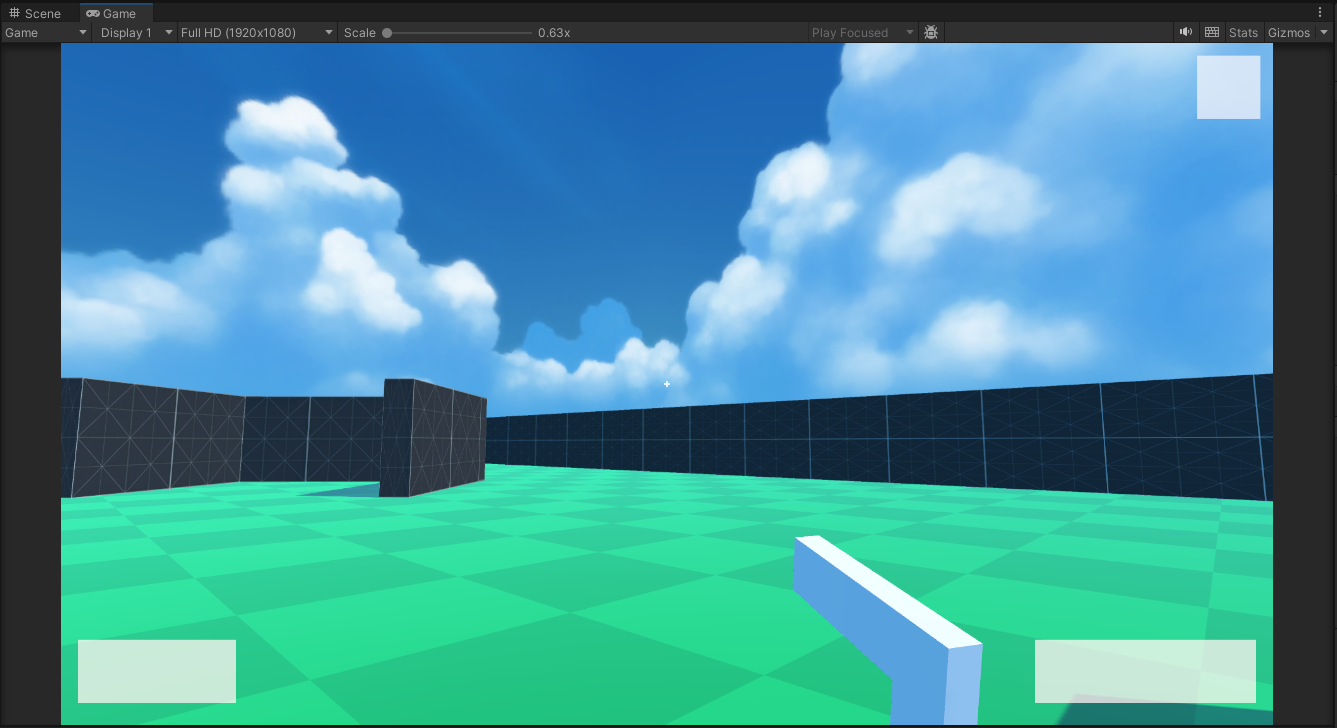
\includegraphics[width=\columnwidth]{weapon}
    \caption{Weapon model and player UI as seen in game.}
    \label{fig:weapon}
\end{figure}

\begin{figure}[ht] 
    \centering
    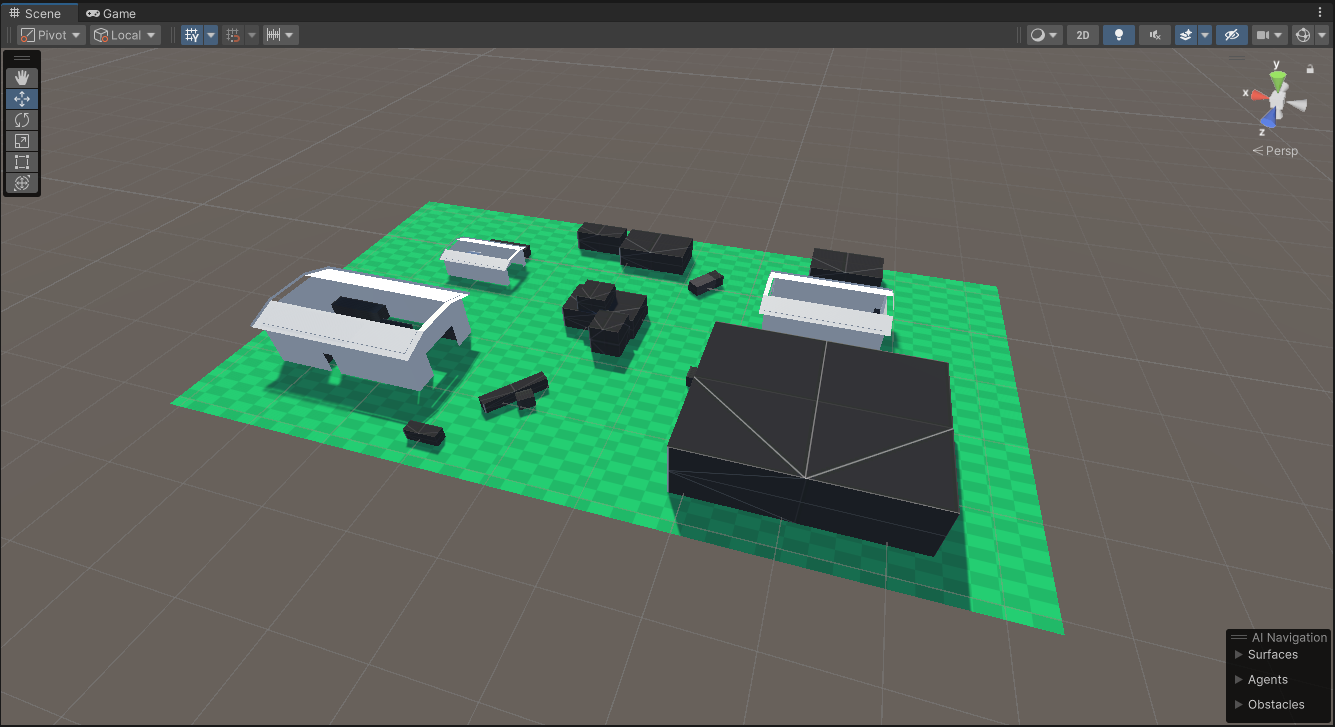
\includegraphics[width=\columnwidth]{farm-map}
    \caption{View of the farm map from above.}
    \label{fig:farm-map}
\end{figure}

\begin{figure}[htb] 
    \centering
    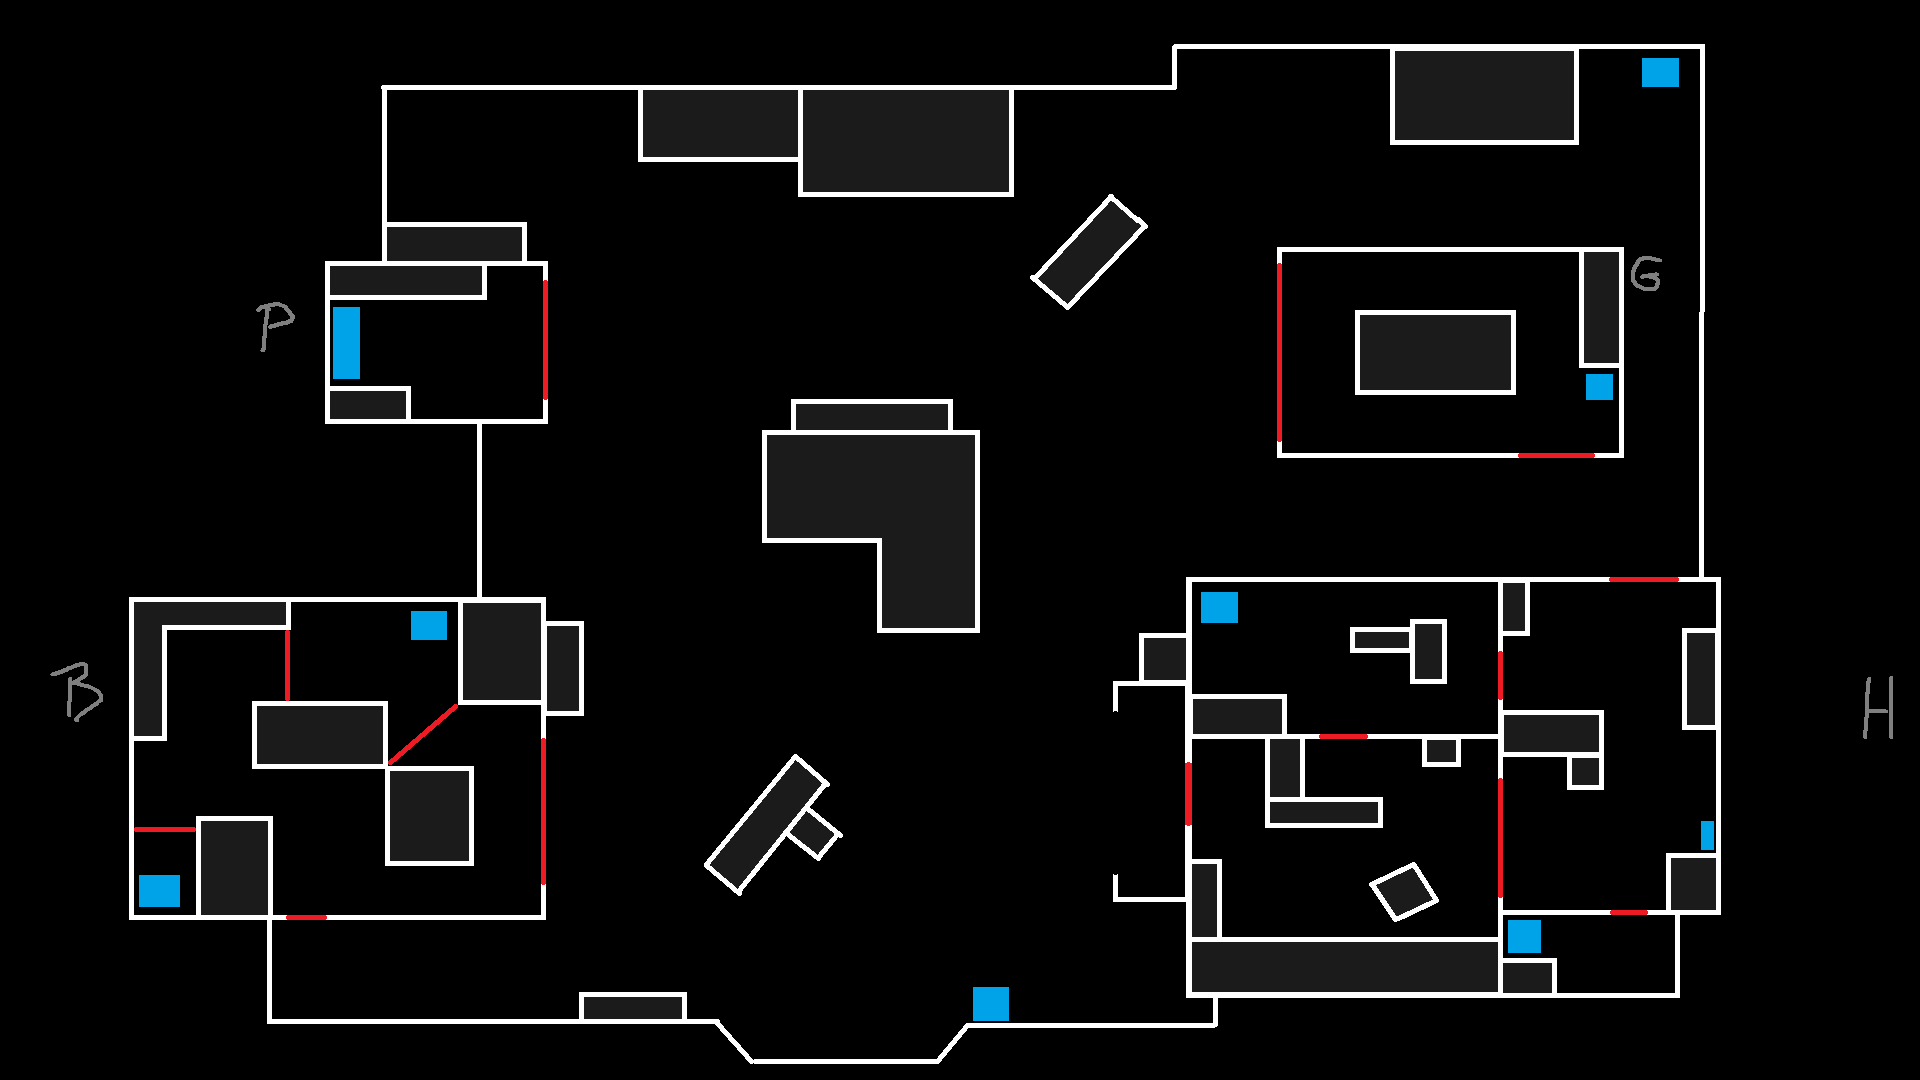
\includegraphics[width=\columnwidth]{farm-bp}
    \caption{Blueprint of the farm map showing its layout.}
    \label{fig:farm-bp}
\end{figure}

\clearpage


\section{Links}
\begin{itemize}
    \item GitHub [https://github.com/zxckv/unity-games-development]
    \item Video [https://www.youtube.com/watch?v=LKCiiVMzX0Y]
\end{itemize}

\clearpage


\end{document}